\documentclass[11pt]{article}
\usepackage{graphicx}
\usepackage{amsmath}
\usepackage[left=3cm,right=1cm,top=1.5cm,bottom=1cm,includeheadfoot]{geometry}




\pagenumbering{gobble}

\begin{document}
\begin{figure}
\includegraphics[scale=.3]{Plot1} \hspace{-.5cm}\includegraphics[scale=.35]{Scan1} $\frac{\text{Slope of rotation}}{\text{length of curve}}= 1.0573$\\ \ \
\includegraphics[scale=.3]{Plot2} \hspace{-.5cm}\includegraphics[scale=.35]{Scan2} $\frac{\text{Slope of rotation}}{\text{length of curve}}= 0.7132$\\
\includegraphics[scale=.3]{Plot3}\hspace{-.5cm}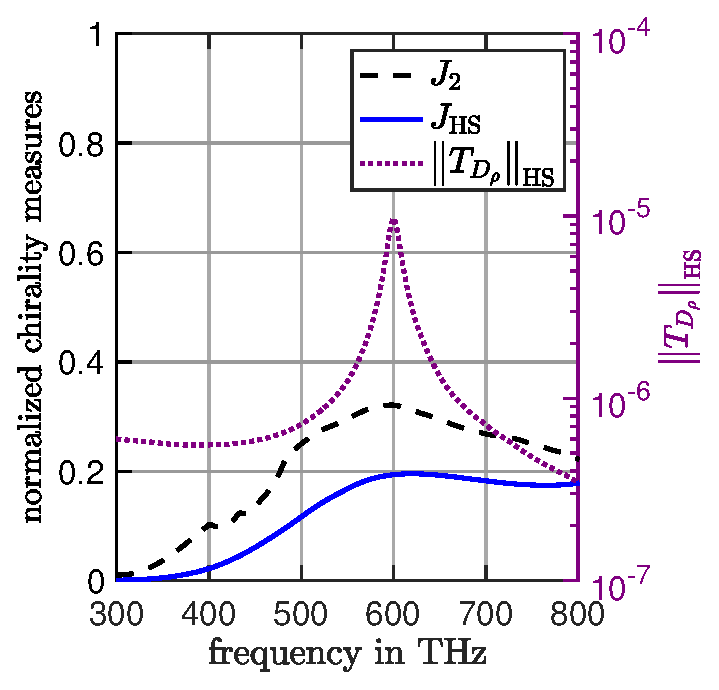
\includegraphics[scale=.35]{Scan3}  $\frac{\text{Slope of rotation}}{\text{length of curve}}= 0.6762$\\
\includegraphics[scale=.3]{Plot4}\hspace{-.5cm}\includegraphics[scale=.35]{Scan4}  $\frac{\text{Slope of rotation}}{\text{length of curve}}=0.6662$\\
\includegraphics[scale=.3]{Plot5}\hspace{-.5cm}\includegraphics[scale=.35]{Scan5}  $\frac{\text{Slope of rotation}}{\text{length of curve}}= 0.6637$\\
\end{figure}
\newpage
\begin{figure}
\includegraphics[scale=.3]{Plot6}\hspace{-.5cm}\includegraphics[scale=.35]{Scan6} $\frac{\text{Slope of rotation}}{\text{length of curve}}= 0.6690$\\
\includegraphics[scale=.3]{Plot7}\hspace{-.5cm}\includegraphics[scale=.35]{Scan7} $\frac{\text{Slope of rotation}}{\text{length of curve}}= 0.6666$\\
\includegraphics[scale=.3]{Plot8}\hspace{-.5cm}\includegraphics[scale=.35]{Scan8} $\frac{\text{Slope of rotation}}{\text{length of curve}}= 0.6661$\\
\includegraphics[scale=.3]{Plot9} \hspace{-.5cm}\includegraphics[scale=.35]{Scan9} $\frac{\text{Slope of rotation}}{\text{length of curve}}= 0.6681$
\end{figure}
\end{document}